% !TeX spellcheck = en_US

\chapter{Validation}\label{chap:check}
In this chapter, the developed framework will be tested.
An input CSAR will be described in section~\ref{sec:inputcsar}.
The processing by the framework is described in section~\ref{sec:process}.
The output CSAR will be added to and displayed by \nameref{subs:wine} in section~\ref{sec:checkwin}.
Generated Artifacts will be checked in section~\ref{sec:checkart}.

\section{Input CSAR}\label{sec:inputcsar}
In this test, an CSAR from the OpenTOSCA Demos is used. 
The CSAR provides a service for Automating the Provisioning of Analytics Tools based on Apache Flink.~\cite{csar_test}
The structure of the service is provided in figure~\ref{fig:winery_source2}. 
The service uses a server virtualization environment named $vSphere$ (The $VSphere\_5.5$ node from the structure.). 
In the environment works the $Ubuntu$ virtual server (The $Ubuntu$-$14.04$-$VM$ node).
The $Ubuntu$ hosts two applications: the $Python$ ($Python\_2.7$) and the $Flink$ $Simple$ ($Flink\_Simple\_1.0.3$).
An analyze shows two external references. The $Python$ node installs the python package and the $Flink$ $Simple$ node - the Java package.
The service has two submodules: a Data Prediction and a Data Delivery, both a hosted on the $Flink$ $Simple$ node and require the Python node. 

\section{Processing}\label{sec:process}
Since the framework is written in the Java, to start it a JDK (version 1.8 or above) is necessary.
Additionally, the apt-get package manager must be installed. 
%For Linux systems it can be easily installed.
To start the framework an Java environment is used.
After the start, a user should enter the input CSAR name, the output CSAR name, and the architecture.
After that, the framework should work fully automatically, analyzing the artifacts and resolving any external references.
Figure \ref{fig:process} provides an example.
\begin{figure}[ht]   
	\centering
	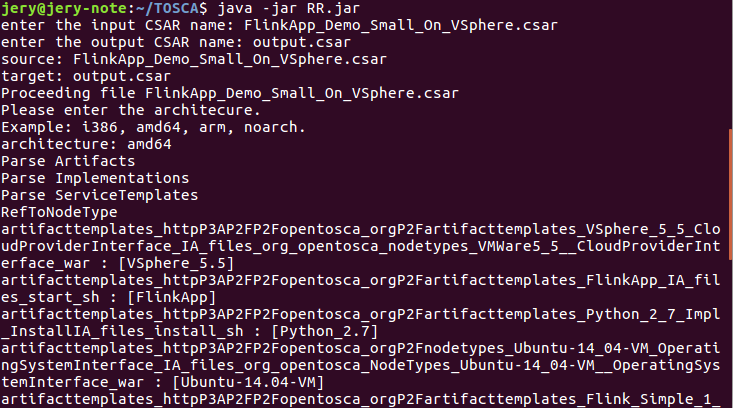
\includegraphics[width=0.7\textwidth]{Screenshot_processing}
	\caption{Processing by the framework.}
	\label{fig:process}
\end{figure}

\section{Displaying with Winery}\label{sec:checkwin}
 \nameref{subs:wine} was installed to test the correctness of the output CSAR. 
 This is an environment for the development of TOSCA systems and is useful for checking the results. \\
 The input CSAR's representation by Winery is displayed in figure~\ref{fig:winery_source2}.
\begin{figure}[ht]   
	\centering
	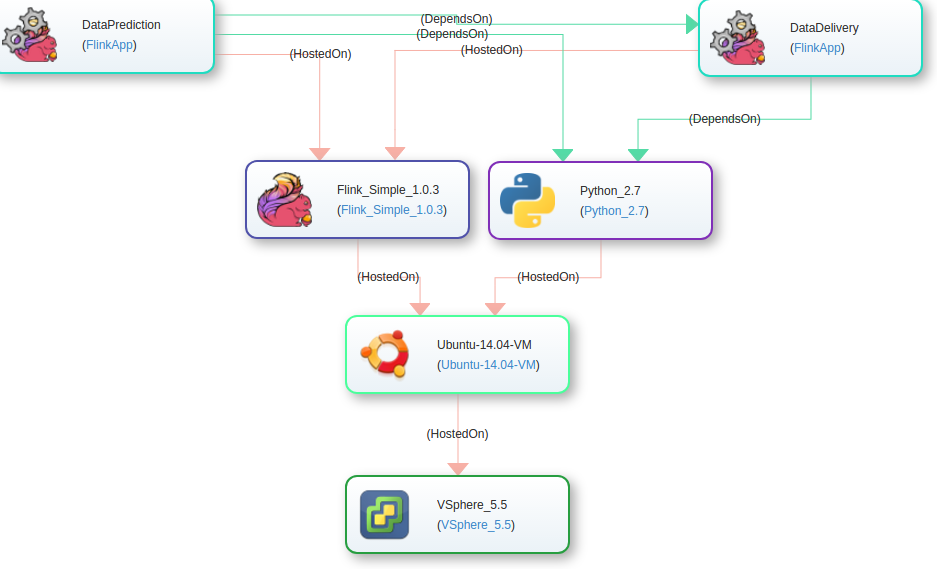
\includegraphics[width=0.7\textwidth]{Screenshot_winery_source2}
	\caption{Source CSAR represented by $Winery$.}
	\label{fig:winery_source2}
\end{figure}
 Those external references will be resolved by the framework and exchanged by new nodes in output CSAR. 
 \subsection*{Add to Winery}
 The output CSAR is added to Winery.
 Due to a significant increase in size, this can be a fairly lengthy procedure.
 It was only six nodes in the input CSAR, but after the processing, the output CSAR contains more than 100 of nodes.
 During the addition to Winery, the CSAR's syntax is tested.
 In a case of errors, messages will be displayed.
 \subsection*{Display by Winery}
 The output CSAR will be displayed.
 Again, due to the high number of nodes, the processing can take a long time. 
 At the time, the correctness of the internal references will be checked.
 If something was defined not properly, these erroneous nodes or links between them will not be displayed.
The representation of the output CSAR by Winery is shown on figure~\ref{fig:winery_output} (Only the part of the CSAR is visible).
\begin{figure}[ht]   
	\centering
	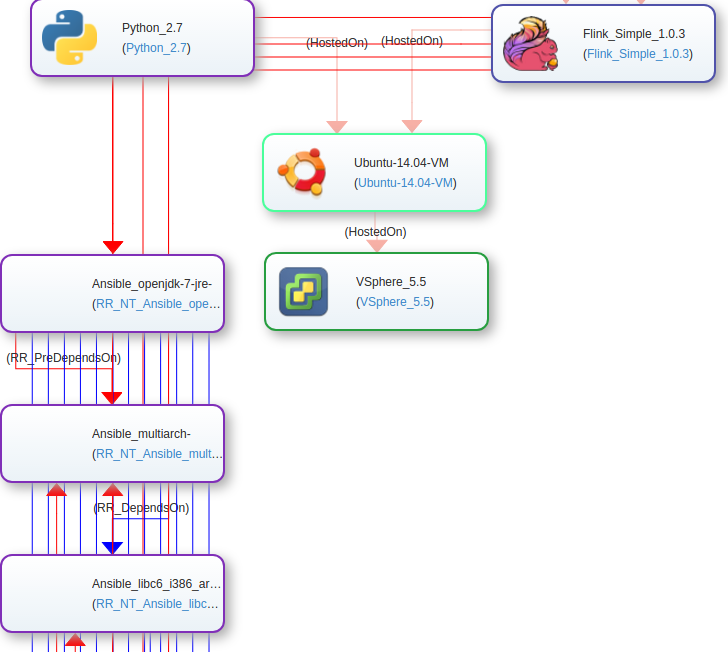
\includegraphics[width=0.7\textwidth]{Screenshot_winery_output}  
	\caption{The output CSAR represented by $Winery$.}
	\label{fig:winery_output}
\end{figure}
 It seems pretty beloved.
 To verify the TOSCA's structure some nodes was moved manually (figure \ref{fig:winery_output2}). 
 \begin{figure}[ht]   
 	\centering
 	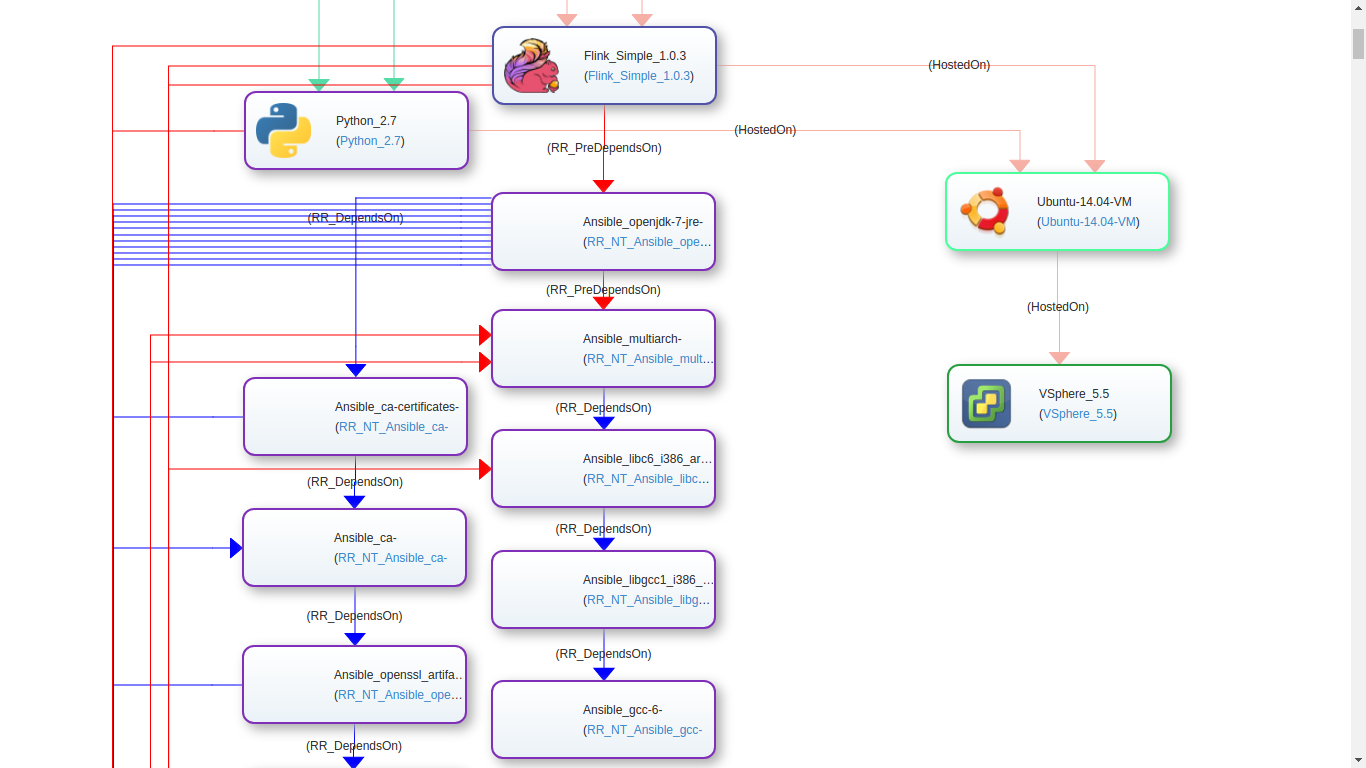
\includegraphics[width=0.7\textwidth]{Screenshot_winery_output2}
 	\caption{The output CSAR represented by $Winery$, some nodes moved manually.}
 	\label{fig:winery_output2}
 \end{figure}
 The correctness of dependencies was verified by checking several nodes with the $apt$-$cache$ $depends$ command.
 By opening the content of the new nodes, it was verified, that there are right artifacts.

\section{Check artifacts}\label{sec:checkart}
Also, it is necessary to check whether it is possible to install new packages using the generated artifacts.
At first bash scripts will be tested, then ansible playbooks.
\subsection*{Check bash scripts}
Since the bash is used in the Linux's command line, it will be pretty easy to check bash installation scripts by starting them (of course that must be done with the necessary privileges).
An example of the $python2.7$ installation is presented in the listing~\ref{lst:check_bash_script}.\\
\begin{Listing}
\caption{Check bash installation script}
\label{lst:check_bash_script}
\begin{lstlisting}
user@user:~$ sudo RR_python2_7-minimal.sh 
(Reading database ... 286091 files and directories currently installed.)
Preparing to unpack python2_7-minimal.deb ...
Unpacking python2.7-minimal (2.7.12-1ubuntu0~16.04.1) over (2.7.12-1ubuntu0~16.04.1) ...
Setting up python2.7-minimal (2.7.12-1ubuntu0~16.04.1) ...
Processing triggers for man-db (2.7.5-1) ...
\end{lstlisting}
\end{Listing}
The process ended without any warnings or errors, which means that it was completed successfully.
This way any bash installation script can be checked.

\subsection*{Check ansible playbooks}
To check an ansible playbook manually we need to extract the zip file containing the playbook. 
During the regular execution, this work will be done by the runtime environment.
The call of the ansible runtime which proceeds the playbook is a simple procedure too.
An example is provided in figure~\ref{fig:ansible_output2}.\\
 \begin{figure}[ht]   
	\centering
	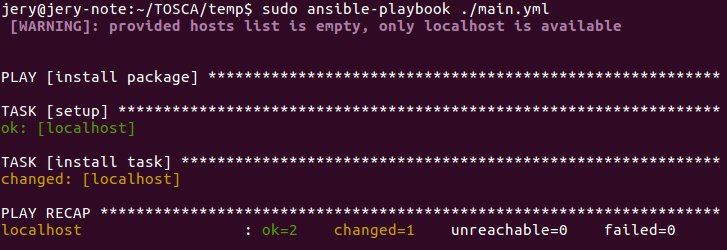
\includegraphics[width=0.7\textwidth]{Screenshot_ansible_output}
	\caption{An ansible playbook's execution process}
	\label{fig:ansible_output2}
\end{figure}
$Ok$ signals that the installation was completed successfully.